% 2009 年四川卷文科第 15 题：各棱长都相等的正三棱柱，M 为 CC_1 的中点。
% 来源 PDF：普通高考/2009/2009四川文.pdf，SHA256 2bb14d3824466d9566238b20ec9270686c67d6e4f2af4186fd22b2a14e633ea7
% 原页：第 1 页（A3 三栏）第 3 栏上部，印刷页 559。
% 重绘依据：正三棱柱竖放，A 左下、B 右下、C 后上；A_1、B_1、C_1 同名加下标；
%   M 在 CC_1 上取中点；AB_1、BM 为异面直线，画细实线；各标注向外避让。
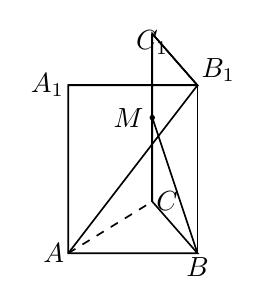
\begin{tikzpicture}[scale=0.82, semithick, every node/.style={inner sep=1.2pt}]
  \coordinate (A) at (0,0);
  \coordinate (B) at (2,0);
  \coordinate (C) at (1.3,0.8);
  \coordinate (A1) at (0,2.6);
  \coordinate (B1) at (2,2.6);
  \coordinate (C1) at (1.3,3.4);
  \coordinate (M) at (1.3,2.1);
  \draw[dashed] (A) -- (C);
  \draw (A) -- (B) -- (C) -- (C1) -- (B1) -- (A1) -- cycle;
  \draw (B) -- (B1);
  \draw (C) -- (C1);
  \draw (A1) -- (B1);
  \draw (B1) -- (C1);
  \draw (A) -- (B1);
  \draw (B) -- (M);
  \fill (M) circle (1.2pt);
  \node[anchor=east] at (A) {$A$};
  \node[anchor=north] at (B) {$B$};
  \node[anchor=west] at (C) {$C$};
  \node[anchor=east] at (A1) {$A_1$};
  \node[anchor=south west] at (B1) {$B_1$};
  \node[anchor=north] at ([yshift=3pt]C1) {$C_1$};
  \node[anchor=east] at ([xshift=-2pt]M) {$M$};
\end{tikzpicture}
